\subsection{Application I/O Interface}\label{subsec:Application_IO_Interface}
The \nameref{def:Operating_System} wants to treat all I/O devices in a standard, uniform way.
Like other complex software-engineering problems, the approach here involves abstraction, encapsulation, and software layering.
Specifically, we can abstract away the detailed differences in I/O devices by identifying a few general kinds, where each is accessed through a standardized set of functions, its \emph{interface}.
The implementation differences are encapsulated in \nameref{def:Kernel_Module}s called \nameref{def:Device_Driver}s that internally are custom-tailored to specific devices but that export one of the standard interfaces.
The software layering used is shown in \Cref{fig:Kernel_IO_Subsystem_Structure}.

\begin{figure}[h!tbp]
  \centering
  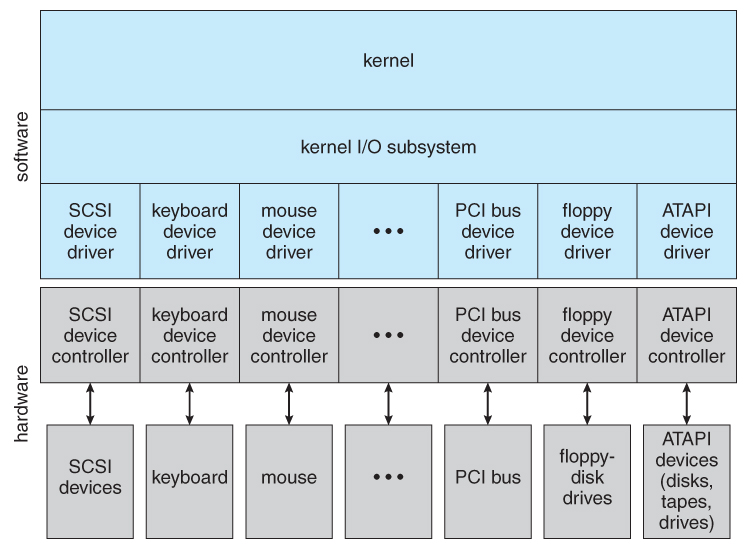
\includegraphics[scale=1.00]{./Drawings/EDAF35-Operating_Systems/Kernel_IO_Subsystem_Structure.jpg}
  \caption{Kernel I/O Subsystem Structure}
  \label{fig:Kernel_IO_Subsystem_Structure}
\end{figure}

This layering methodology is used to hide differences among devices and their controllers from the \nameref{def:Kernel}'s I/O subsystem.
This is analogous to the I/O system calls encapsulating the behavior of devices in a few generic classes that hide hardware differences from applications.

Making the I/O subsystem independent of the hardware simplifies the job of the operating-system developer.
It also benefits the hardware manufacturers.
They either:
\begin{itemize}[noitemsep]
\item Design new devices to be compatible with an existing host controller interface.
\item Write device drivers to interface the new hardware to popular operating systems.
\end{itemize}


%%% Local Variables:
%%% mode: latex
%%% TeX-master: "../../EDAF35-Operating_Systems-Reference_Sheet"
%%% End:
